\section{A Simple LED Circuit}
\label{sec:LED}

	\subsection{Setting up the circuit}
	
		Let's start off with a simple circuit. Firstly, we'll always shut down and \textbf{unplug} our Pi before we begin connecting to the GPIO.
		
		We will build our circuit using a breadboard. Breadboards have conductive wire underneath their circuits, which form `lanes'. You can see these wires in figure \ref{fig:pinout_breadboard}.
	
		\begin{figure}[h]
			\centering
			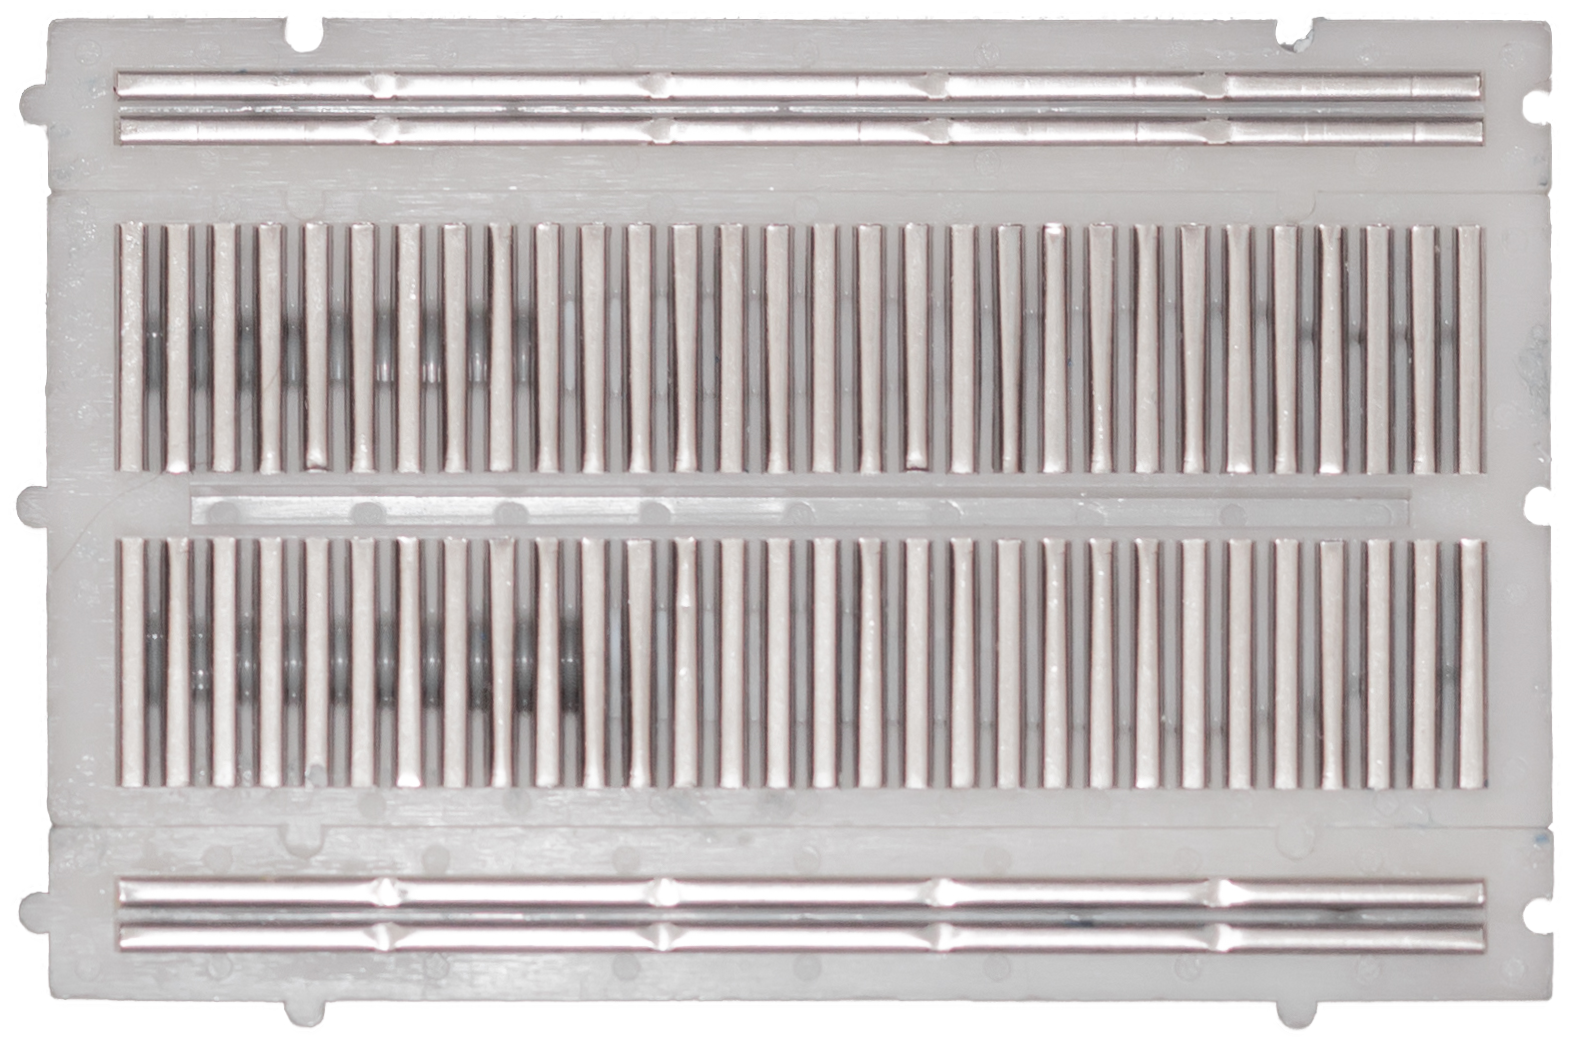
\includegraphics[width=0.7\linewidth]{McrRaspJam/011_Motors/1_LED/breadboard_underside}
			\caption{The underside of a breadboard, showing the direction of electrical connections.}
			\label{fig:pinout_breadboard}
		\end{figure}
	
		We will use the positive and negative bus `lanes' like the ends of a battery in a simple electronic circuit, current starts at the positive end, and travels through components to the negative end.
		
		To make a complete circuit, we will connect these lanes to the Pi's GPIO.
		
		\begin{enumerate}[noitemsep]
			\item \textbf{Connect} the positive bus to the 3V3 pin on the Raspberry Pi with a jumper cable.
			\item \textbf{Connect} the negative bus to one of the GND pins with another jumper cable.
		\end{enumerate}
	
		By convention, you should use a red cable for the positive terminal and black for the negative terminal.
		
		\begin{enumerate}[noitemsep]
			\setcounter{enumi}{2}
			\item \textbf{Place} the LED across the gap in the centre of the breadboard, a pin on each side.
			\item Use a Jumper cable to \textbf{connect} the positive bus to the positive leg of the LED.
			\small
			\begin{itemize}[noitemsep]
				\item The LED is a Diode, so only lets current through one way.
				\item the positive leg (anode) of the LED is the longer of the two legs.
			\end{itemize}
			\normalsize
		\end{enumerate}
		
		We will now need to complete the circuit by connecting the negative pin of the LED.
		
		However, the LED will try and take a lot of power. To prevent it from burning out the Raspberry Pi, we'll add a resistor to limit the current flowing through the LED.
		
		\begin{enumerate}[noitemsep]
			\setcounter{enumi}{4}
			\item \textbf{Insert} the resistor in the lane where the negative LED leg is placed, and bridge it to any other lane.
			\item \textbf{Connect} this lane back to the negative bus with a jumper cable.
		\end{enumerate}
		
		\begin{figure}[h]
			\centering
			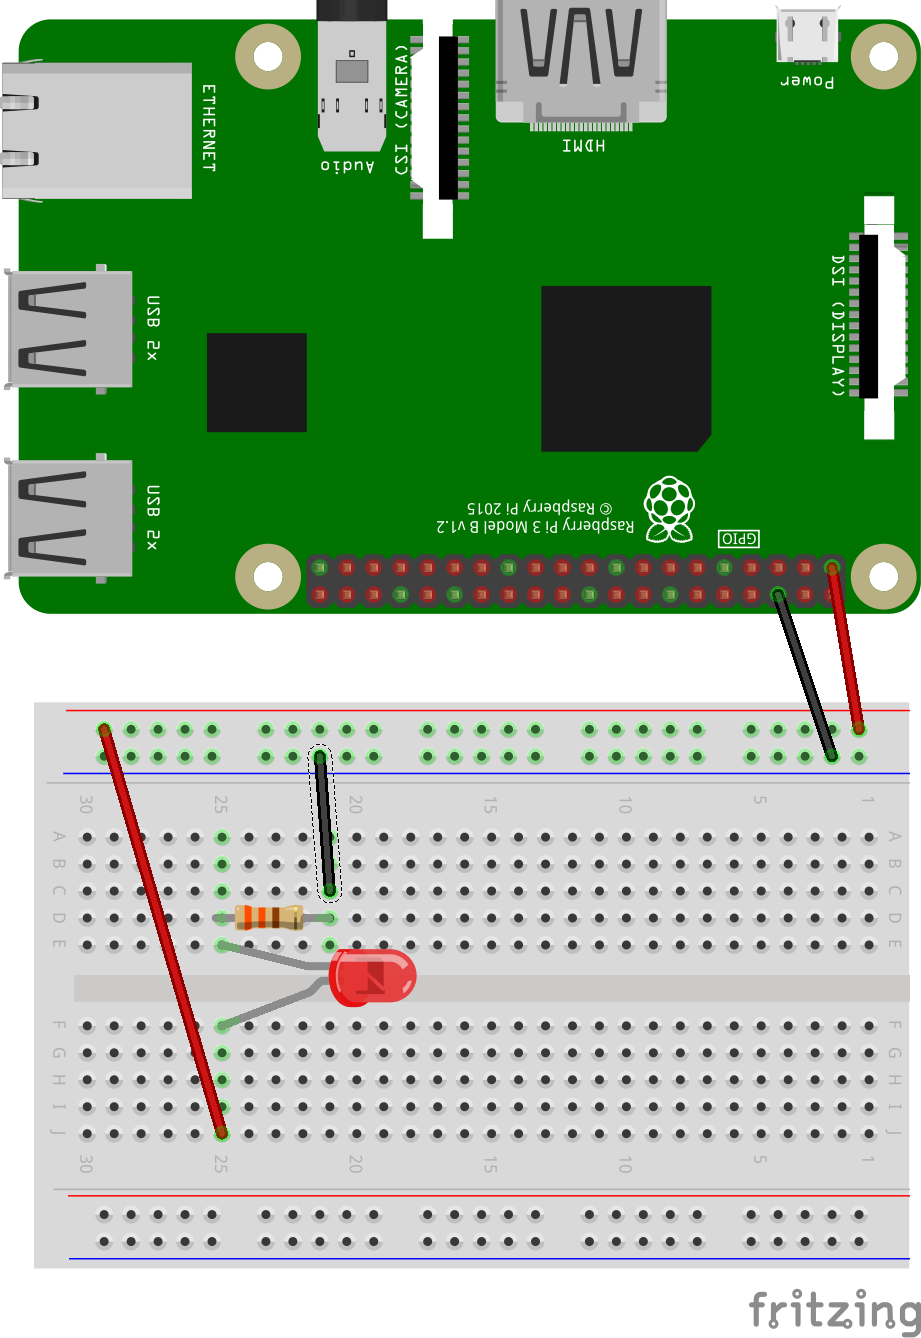
\includegraphics[width=0.7\linewidth]{McrRaspJam/011_Motors/1_LED/schematic_LED_3}
			\caption{The complete LED circuit}
			\label{fig:schematic_LED_3}
		\end{figure}
		
		Once you're happy your circuit matches figure \ref{fig:schematic_LED_3}, you can try turning on your Raspberry Pi. If everything is correctly connected, your LED will light up!
		
	\subsection{Modify for GPIO}
	
			Our LED is currently connected to a constant 3.3 volt supply, so we are unable to turn the LED off without unplugging the whole Pi. To control the LED through code, we need to use a GPIO pin.
	
			\begin{enumerate}[nosep]
				\item Remember to shut down and \textbf{unplug} your Pi first.
				\item \textbf{Remove} the two red cables that were supplying the 3V3 voltage.
				\item Use a jumper cable to \textbf{connect} GPIO pin 23 to the positive pin of the LED.
			\end{enumerate}	
		
			\begin{figure}[h]
				\centering
				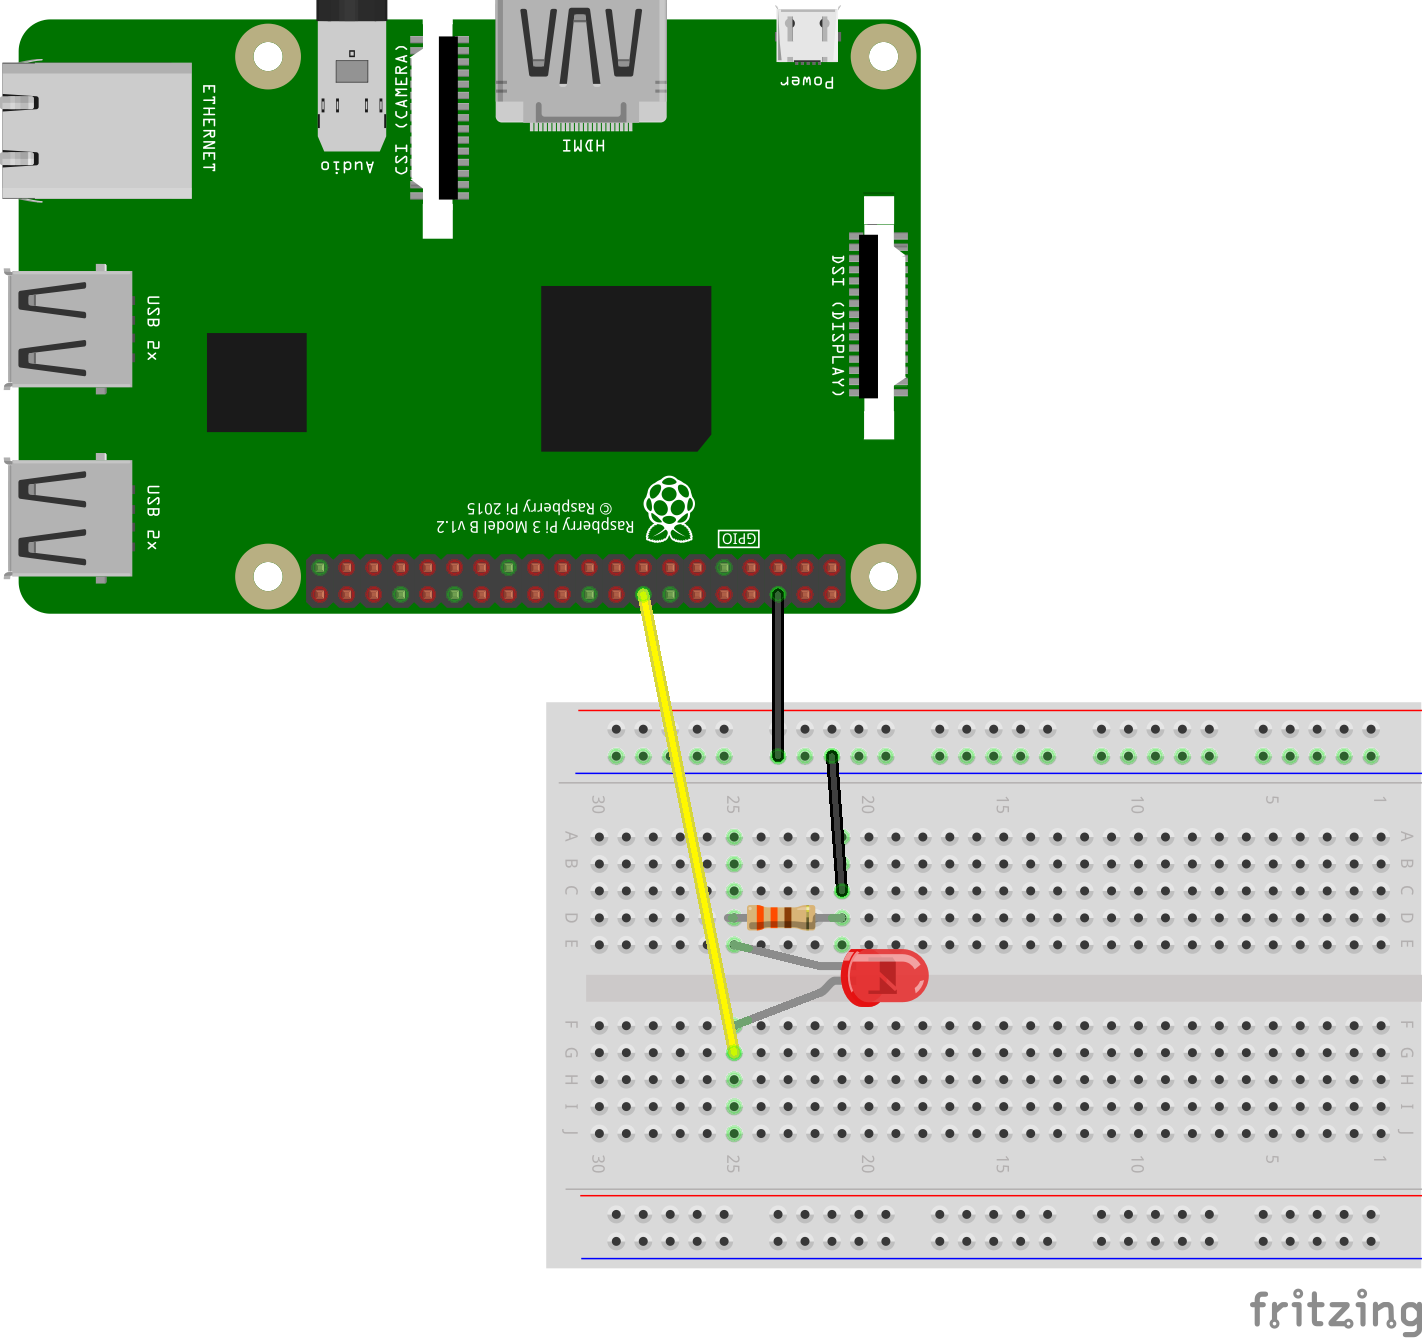
\includegraphics[width=0.7\linewidth]{McrRaspJam/011_Motors/1_LED/schematic_LED_4}
				\caption{A GPIO controlled LED circuit}
				\label{fig:schematic_LED_4}
			\end{figure}
		
	\subsection{Programming the LED}
		
			Once again, if you're happy your circuit matches figure \ref{fig:schematic_LED_4}, you can start up your Raspberry Pi again.
			The LED will be off to begin with, so we will write a simple Python program to turn the LED on.
			
			Once your Pi is started up, start \textit{IDLE 3} and open the template python file for this workshop.
		
			\lstinputlisting[style=Python, lastline=6]{McrRaspJam/011_Motors/1_LED/0_LED.py}
			
			Add the following lines into this file:
			
			\lstinputlisting[style=Python, firstline=7, firstnumber=7, lastline = 10]{McrRaspJam/011_Motors/1_LED/0_LED.py}
			
			Before we control something through GPIO, we need to setup the pin. We just stated that pin 16 (labelled `LED') is an output device, i.e. we are outputting a signal to the light, we aren't reading a sensor input.
			
			Note the pin number is 16, not 23. We plugged into GPIO pin 23, but some pins on this block have other functionalities, but are still numbered. (See Appendix \ref{sec:pinout} for full pinout)
			
			Now it is set up, we can control the GPIO pin:
			
			\lstinputlisting[style=Python, firstline=11, firstnumber=11, lastline = 13]{McrRaspJam/011_Motors/1_LED/0_LED.py}
			
			Once again, we are sending a command for pin number 16 (`LED'), this time telling it to output a `high' signal. This will turn on our LED.
			
			Let's have our LED on for a few seconds, then turn it off before the program ends. The function sleep() will cause the program to wait, then we will repeat the GPIO.output() function, this time using GPIO.LOW to turn off the LED.
			
			\lstinputlisting[style=Python, firstline=14, firstnumber=14, lastline = 20]{McrRaspJam/011_Motors/1_LED/0_LED.py}
			
			We place GPIO.cleanup() at the end of our program, to reset the pin setup for the next program.
			
			You can now try running your program.
		
